\section{Architecture overview}

The ABEL library can be splitted into a Frontend and a Backend part.
The frontend provides the main API, which is completely agnostic of the actual storage engine, 
whereas the backend provides a framework and some implementations to adapt ABEL to a specific storage engine.
The boundary between Backend and Frontend can be drawn straight through the deferred class REPOSITORY.

\subsection{Frontend}

If you've read the previos part of the documentation, then you should be quite familiar now with the frontend.
The main classes are:
 \begin{itemize}
  \item CRUD\_EXECUTOR: Provides features for CRUD operations, and does some error handling for transaction conflicts.
  \item QUERY: Collects information like the Criteria, Projection, and (through its generic parameter) the type of the object to be retrieved. It doesn't do anything by itself.
  \item TRANSACTION: Represents an ABEL transaction, and is responsible to internally propagate errors. It provides the features commit and rollback, but internally it relies on REPOSITORY to execute them.
  \item CRITERION: Its descendants provide a filtering function for retrieved objects, and it has builtin functions to generate a tree of criteria using the overloaded logical operators.
 \end{itemize}

You can see that the main objective of the frontend is to provide an easy to use, backend-agnostic API, and to collect information that the backend can consume.

\todo{Insert class diagram}


\subsection{Backend}

The frontend needs a repository which is specific to a data storage engine, and the backend provides a framework to implement these repositories (in cluster Framework).
There are also some already predefined repositories inside the backend (cluster Backends), like the IN_MEMORY_REPOSITORY.

Inside the framework, there are basically three layers of abstraction. The first is the deferred class REPOSITORY, which is still very object-oriented:
It takes Eiffel objects that may have a big object graph attached, and returns such fully loaded objects. 
It also provides some fine-grained control to restrict depth in an object graph.

The second important level of abstraction is the deferred class BACKEND_STRATEGY, which deals only with one object at once. 
The layer in between REPOSITORY and BACKEND_STRATEGY take care of disassembling the object graph into single objects, wrapped in a more explicit notion of the object graph. 
You can read in the object-relational mapping section ~\ref{section:ORM} how this is exactly done.
Anyway, the BACKEND_STRATEGY only knows the concept of a single object and of a collection, and it is responsible to map these to the actual persistence mechanism, e.g. a database with a specific layout. 

The third layer of abstraction is a set of wrappers to a database. It only wraps the connection details, and has functions to execute SQL and retrieve the result in a standardized way.
It is very useful if you want to easily swap e.g. from a MySQL database to SQLite, but it's abstraction is not perfect - i.e. it doesn't take into account the different SQL variations.



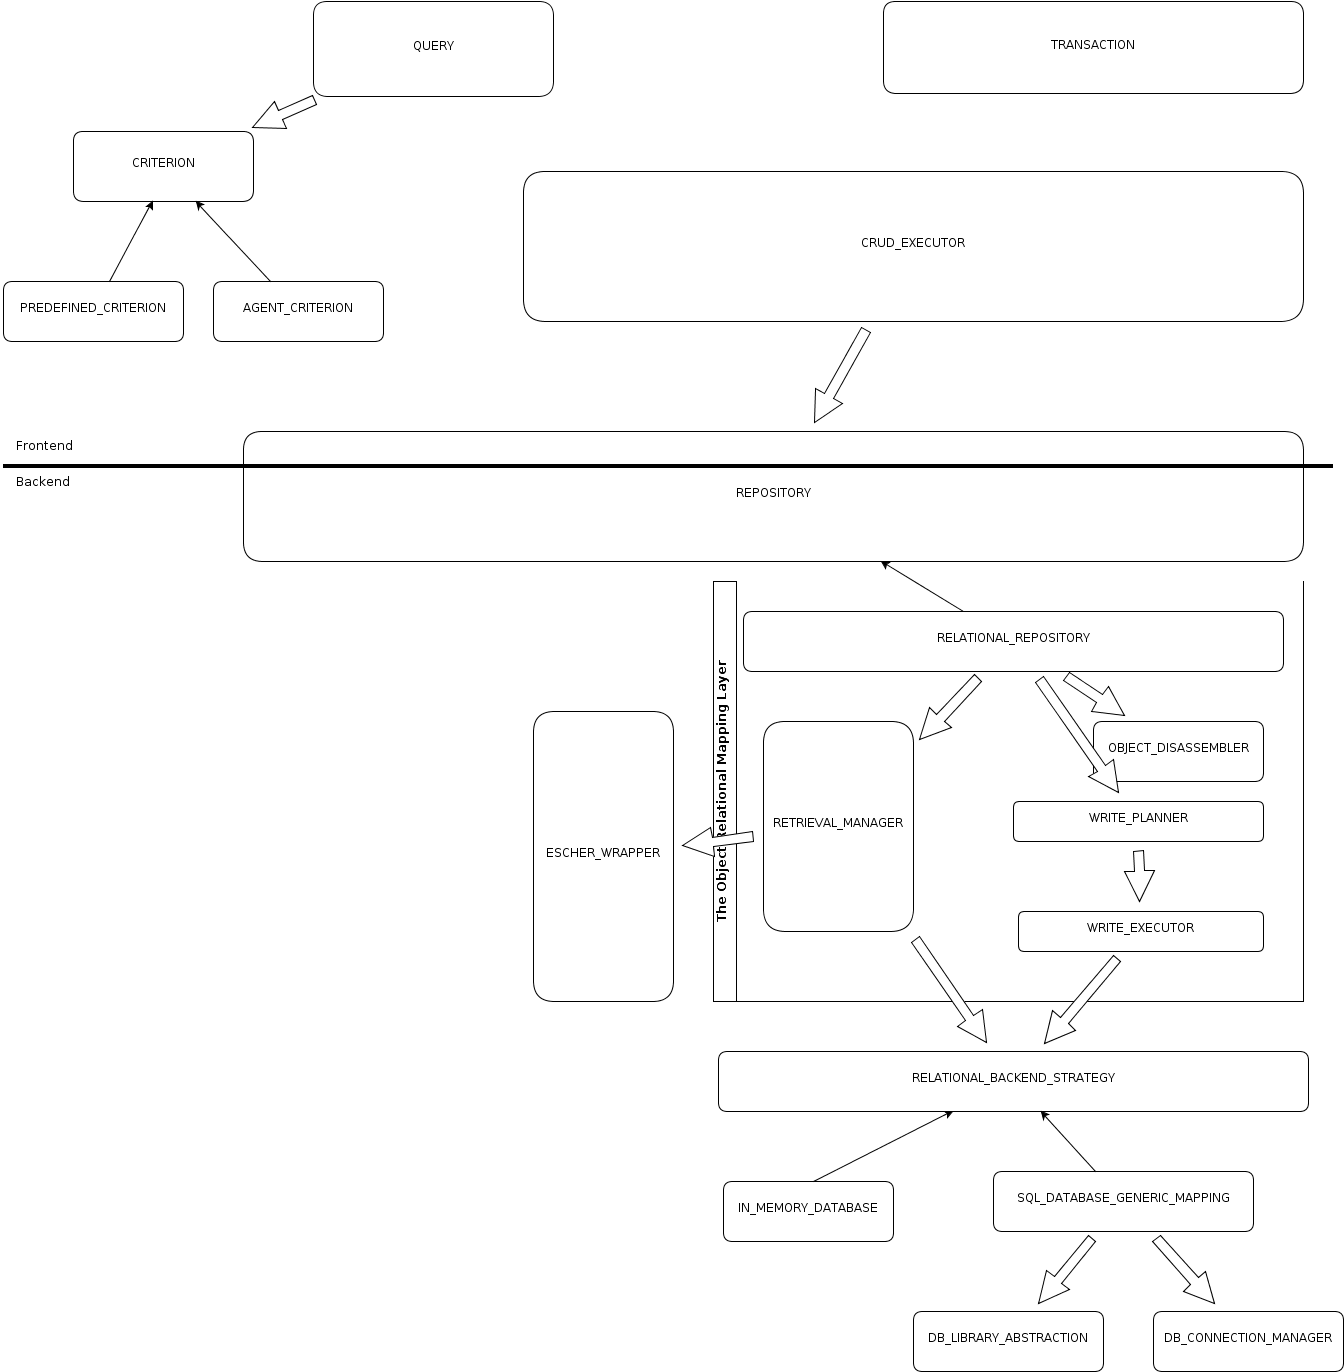
\includegraphics[width = 13cm] {class_diagram.png}

\section{Object-relational Mapping}
\label{section:ORM}

\subsection{Object graph settings}


\section{Backend abstraction}

\subsection{REPOSITORY}

\subsection{BACKEND\_STRATEGY}

\subsection{Database wrapper}


\section{Extensions}

\section{Adaption to a specific database layout}


\section{Limitations of the library}
TODO

Current limitations:
\begin{itemize}
\item Not all features available if adapted to a custom DB layout 
\item Inheritance currently not properly supported (due to limitation of INTERNAL)
\item Reals have rounding error
\item No ordering support (at least not yet)
\item
\end{itemize}

%What exactly has to be here? Is a missing feature (like ordering support) a limitation as well?


TODO

%\section{ PART 2: Technical Documentation}

%\subsection{Moved to technical documentation}
%about criteria
%It will internally build a tree of criteria, with specialized AND, OR or NOT instances as nodes and the usual predefined or agent instances as leafs.


%\subsubsection{Performance remarks}

%ABEL will try to let the backend do as much of the filtering as is possible, to reduce the overhead of e.g. network communication or building unnecessary objects.
%This especially means that ABEL will compile predefined queries to SQL if you have a relational database as a backend. 
%However, if there is an agent criterion OR-ed to a predefined criterion, the test can not be made in the database because you might get false negatives.
%Therefore, to have optimal performance, you should consider the following points:

%\begin{itemize}
%\item Try not to use agent criteria if you have a relational database backend.
%\item Try not to use OR on agent criteria.
%\item Try to keep OR-ed agent criteria as deep down the tree as possible (as the above OR-node defaults to true and thus is not checked for in the backend)
%\end{itemize}
